% Created:  Fri 04 Jul 2014 04:47 PM
% Modified: Fri 11 Jul 2014 11:15 AM
% @author Josh Wainwright
% File name : imagej_plugin.tex

\section{ImageJ Plugin}
\label{sec:imagej_plugin}

The first version of the plugin simply allowed the user to visualise the data,
once it had been processed and entered into a quadtree. Though this provided
little benefit to the researcher producing data, it can be useful to simply get
an insight into the process that a program is using to analyse one's data so
that the results can be better interpretted. For this reason, this version
served as a foundation for later versions of the plugin so that, when loading
data, a user gets the opportunity to view the data before proceding with the
analysis.

The analytical steps that are undertaken are descibed in more detail in later
sections.

The code used to generate this view of the data was modified to make use of the
easy image generation functions present in ImageJ. Now, instead of many
different objects being manipulated for each view of the data, a single array
with a value for each pixel is needed. For the cases where the user wishes to
view the clusters that have been found, but not have them affect the image, the
image is created with a number of different \emph{slices} in the image
\emph{stack}. Slices are ImageJ's representation of images with two or more
layers, or alternative views, each of which resides in a stack of slices. Each
slice in a stack must have the same dimensions.

\begin{figure}[tbhp]
\begin{figure*}[tbhp]
	\centering
	\includegraphics[width=0.8\linewidth]{imagej-stacks.pdf}
	\caption{imagej-Stacks}
	\label{fig:imagej-stacks}
\end{figure}

\begin{figure}[tbhp]
    \centering
    \begin{subfigure}[c]{0.48\linewidth}
        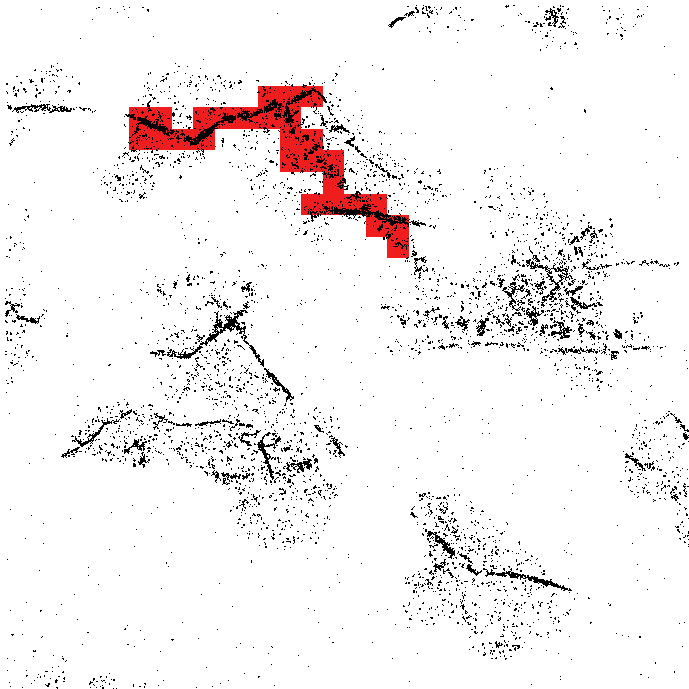
\includegraphics[width=\textwidth]{single-cluster.png}
        \caption{}\label{fig:single-cluster-points}
    \end{subfigure}%
    \quad
    \begin{subfigure}[c]{0.48\linewidth}
        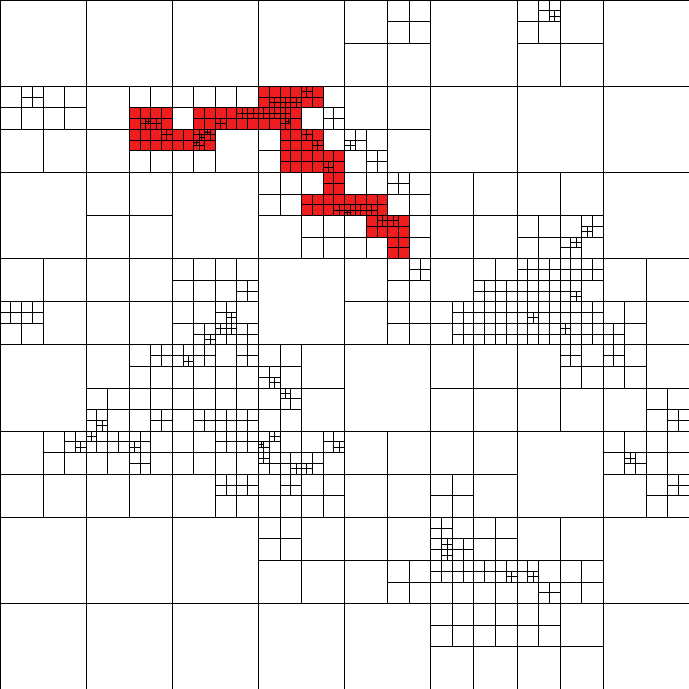
\includegraphics[width=\textwidth]{single-cluster-lines.png}
        \caption{}\label{fig:single-cluster-lines}
    \end{subfigure}
	% TODO caption
    \caption{} \label{fig:single-cluster}
\end{figure}
